% 原书印刷207--218页，PDF物理231--242页，完整章末.
\subsection{讨论}\label{sec:5.5}

\subsubsection[无穷阶Wasserstein距离]{$W_\infty$距离}\label{sec:5.5.1}\index{0003@$L^\infty$传输成本（$L^\infty$ transport cost）|hyperpage}

$W_p$定义中的$p=\infty$情形值得特别注意. 容易想到如何在概率测度上定义$W_\infty$距离：
\[
W_\infty(\mu,\nu):=\inf\{\|x-y\|_{L^\infty(\gamma)}:\gamma\in\Pi(\mu,\nu)\},
\]
其中右端的极小化问题正是\autoref{sec:3.2}研究的问题. 与本章其他部分一样，这里的区别是：不着重考察最优映射，而主要将最优成本看作两个测度的函数，并用作概率测度空间上的距离.

为恰当定义$W_\infty(\mu,\nu)$，应限制在有界支撑测度空间$\mathscr P_\infty(\Omega)$. 否则，某些测度对之间可能不存在具有有界位移的方案$\gamma$. 由\autoref{sec:3.2}的结果，若$\mu\ll\mathscr L^d$，则$W_\infty(\mu,\nu)$也等于
\[
\inf\{\|\mathrm T(x)-x\|_{L^\infty(\mu)}:\mathrm T_\#\mu=\nu\}.
\]
不难验证预期的性质
\[
W_\infty(\mu,\nu)=\lim_{p\to\infty}W_p(\mu,\nu),
\]
其中右端关于$p$递增（证明留作\autoref{ex:35}）. 在$W_p$相应的三角不等式中令$p$取极限，就能证明三角不等式.

注意，在一维中，由\autoref{sec:2}的结果，对每个$p<\infty$及成本$|x-y|^p$，移动粒子的最优方式都是单调递增映射. 取极限后，这也是$L^\infty$问题的最优映射.

一般而言，得到紧集上概率测度的一种新距离，它度量从一个分布移动到另一个分布所需的最小最大粒子位移. 有趣的是，虽然产生这一距离的建模方式与$p<\infty$时相同，诱导的拓扑却完全不同.

事实上，取不同的点$x,y\in\Omega$及不同的$s,t\in[0,1]$，容易验证
$W_\infty((1-t)\delta_x+t\delta_y,(1-s)\delta_x+s\delta_y)=|x-y|$.
特别地，概率测度$(1-t)\delta_x+t\delta_y$在$t\to0$时不趋于$\delta_x$，尽管对所有距离$W_p$乃至测度的强收敛都有收敛. 实际上，即使$\Omega$紧，只要$\Omega$的基数大于$1$，空间$(\mathscr P(\Omega),W_\infty)$就既不紧，也不可分.

另一方面，通过存在满足$\|\mathbf v_t\|_{L^\infty(\mu_t)}\le|\mu'|_{W_\infty}(t)$的速度场$\mathbf v_t$来刻画Lipschitz曲线，仍然成立；令$p\to\infty$，即可容易地从\autoref{obj:5.14}推出. 这一事实连同对$W_\infty$的Lipschitz曲线的广泛使用，被\cite{b79}用于分析分支运输的一个替代模型. 尽管该模型的作用很有限，其中一些例子与讨论仍有助于理解Wasserstein空间的结构.

不过，距离$W_\infty$在许多建模问题中自然出现，对分析非常不同的现象十分有用. 最早使用这一距离的论文之一是研究旋转恒星形状的\cite{b232}. 该文选择$W_\infty$的动机是以下观察（将在\autoref{sec:7.4.3}更充分展开）：测度$\mu$是某个泛函$F$在$\mathbb W_\infty$中的局部极小点，当且仅当每个$x\in\operatorname{spt}(\mu)$都满足某个函数$f$的局部极小性条件（$f$等于$F$的一阶变分，见\autoref{sec:7.2}）. 将$W_\infty$替换为$W_p$，这一等价性便失效.

最后，值得一提的是$W_\infty$与$W_p$之间一个反向不等式（无法由\eqref{eq:5.1}推出），形如
\[
W_\infty(\mu,\nu)\le C W_p(\mu,\nu)^{p/(p+d)},
\]
其中常数$C$依赖于$p$、维数$d$、区域$\Omega$以及$\mu$密度的一个下界. 这一不等式来自\cite{b74}证明的更强结果：若$\mu=f\cdot\mathscr L^d$，$f\ge a>0$，$\mathrm T$为从$\mu$到另一测度$\nu$的最优运输映射，则
\[
\|\mathrm T-\mathrm{id}\|_{L^\infty}^{p+d}
\le C(\Omega,p,d)\int_\Omega|\mathrm T(x)-x|^p\,dx
\le\frac{C(\Omega,p,d)}a\int_\Omega|\mathrm T(x)-x|^p\,d\mu(x).
\]
证明利用$\mathrm T$的$c$-循环单调性条件，保证每当固定满足$|\mathrm T(x)-x|>0$的点$x$时，$x$附近存在某个区域$R$，体积正比于$|\mathrm T(x)-x|^d$，使每个$y\in R$的距离$|\mathrm T(y)-y|$都不小于$|\mathrm T(x)-x|$的某个固定比例.

\subsubsection{Wasserstein距离与负Sobolev距离}\label{sec:5.5.2}\index{D045@对偶范数（dual norms）|hyperpage}

已经注意到，距离$W_1$由一个范数诱导，它是Lipschitz半范数的对偶. 事实上，若考虑赋有范数$\|f\|:=\operatorname{Lip}(f)$的零均值Lipschitz函数空间$\mathscr X$，则$\mathscr P_1(\Omega)$上的距离$W_1$恰好是拓扑对偶$\mathscr X'$的范数所对应的距离. 有趣的是，赋予这一距离的概率测度空间完备，但赋予同一范数的有限测度空间并不完备. 更准确地，可以考虑赋予范数$\|\varrho\|:=\sup\{\int f\,d\varrho:f\in\operatorname{Lip}_1(\Omega)\}$的零均值有限标量测度，再考察其完备化. 注意，序列$\varrho_n:=\sum_{i=1}^n\delta_{1/2i}-\delta_{1/(2i-1)}$对该范数是Cauchy列，但其极限为Dirac质量的无穷和，并非有限标量测度. \cite{b73}研究了测度集合对这一范数的完备化，证明它等同于$L^1$向量场的散度所组成的分布集合. 这一漂亮结果与\autoref{sec:4}研究的$L^1$-Beckmann问题建立了有趣联系.

无论如何，既然已经明确距离$W_1$在与$W^{1,\infty}$函数的对偶中的作用，就会问其他距离$W_p$是否与形如$W^{1,q}$的Sobolev空间对偶（例如$q=p'=p/(p-1)$）. 答案显然是“否”，因为并非所有概率测度都属于对偶空间$W^{-1,p}$（特别地，只有$W^{1,q}$中的函数连续，即$q>d$时，Dirac质量才属于其对偶）. 不过，存在一些部分答案和类比. 例如，以下引理曾为不同目的分别在\cite{b214}及后来的\cite{b225}中得到证明.

\begin{lemma}\label{obj:5.33}
假设$\mu$与$\nu$是凸区域$\Omega$上的绝对连续测度，密度均由同一个常数$C$控制. 则对每个函数$\phi\in H^1(\Omega)$，有
\[
\int_\Omega\phi\,d(\mu-\nu)\le\sqrt C\,\|\nabla\phi\|_{L^2(\Omega)}W_2(\mu,\nu).
\]
\end{lemma}
\begin{proof}
设$\mu_t$为$\mu$与$\nu$之间的常速测地线，$\mathbf v_t$为由\autoref{obj:5.14}联系于该曲线的速度场. 则$(\mu,\mathbf v)$满足连续性方程，且$\|\mathbf v_t\|_{L^2(\mu_t)}=W_2(\mu,\nu)$. 利用$\mu_t$对所有$t$都绝对连续、且其密度由同一常数$C$控制这一事实；它将在\autoref{sec:7}证明（\autoref{obj:7.29}）. 因而
\[
\begin{aligned}
\int_\Omega\phi\,d(\mu-\nu)
&=\int_0^1\frac d{dt}\left(\int_\Omega\phi(x)\,d\mu_t(x)\right)dt
=\int_0^1\int_\Omega\nabla\phi\cdot\mathbf v_t\,d\mu_t\,dt\\
&\le\left(\int_0^1\int_\Omega|\nabla\phi|^2\,d\mu_t\,dt\right)^{1/2}
\left(\int_0^1\int_\Omega|\mathbf v_t|^2\,d\mu_t\,dt\right)^{1/2}\\
&\le\sqrt C\,\|\nabla\phi\|_{L^2(\Omega)}W_2(\mu,\nu),
\end{aligned}
\]
证明完成.
\end{proof}

\phantomsection\label{idx:root5-p210-hminusone}\index{0001@$H^{-1}$范数（$H^{-1}$ norm）|hyperpage}这里不展开不同于$p=p'=2$的指数情形，因为二次情形似乎最有意义（一般情形见\autoref{ex:38}）. 二次情形中出现的确切负Sobolev范数为$\dot H^{-1}$范数，值得作些说明. 先定义
\[
\|\mu-\nu\|_{\dot H^{-1}(\Omega)}
=\sup\left\{\int\phi\,d(\mu-\nu):\|\nabla\phi\|_{L^2}\le1\right\}.
\]
注意还有$\|\mu-\nu\|_{\dot H^{-1}(\Omega)}=\|\nabla u\|_{L^2}$，其中$u$为Neumann问题
\[
\begin{cases}-\Delta u=\mu-\nu&\text{在 }\Omega\text{ 内},\\
\dfrac{\partial u}{\partial\mathbf n}=0&\text{在 }\partial\Omega\text{ 上}
\end{cases}
\]
的解. 事实上，对这样的$u$，有$\int\phi\,d(\mu-\nu)=\int\nabla\phi\cdot\nabla u\le\|\nabla\phi\|_{L^2}\|\nabla u\|_{L^2}$，且$\phi=u/\|\nabla u\|_{L^2}$时取等号. 还能看出
\[
\|\mu-\nu\|_{\dot H^{-1}(\Omega)}=\min\{\|\mathbf w\|_{L^2}:\nabla\cdot\mathbf w=\mu-\nu\},
\]
因为这一极小化问题中的最优$\mathbf w$为梯度（见\autoref{sec:4.4.1}及关于问题\eqref{eq:4.27}的讨论），且$\mathbf w=-\nabla u$.

\phantomsection\label{idx:root5-p211-crowd}\index{0002@$L^\infty$密度约束（$L^\infty$ density constraints）|hyperpage}\index{C032@人群运动（crowd motion）|hyperpage}对距离$W_2$与$\dot H^{-1}$之间关系的研究如今十分活跃（这里$\dot H^{-1}$表示连通区域上赋以梯度$L^2$范数的零均值$H^1$函数空间$\mathscr X$的对偶），因为当所涉密度接近$\varrho=1$时，这两种距离渐近等价. 在拥挤带来$L^\infty$约束$\varrho\le1$的演化问题中，例如人群运动（见\autoref{sec:8.4.2}），这正是相关情形. 通过一些一般估计，可以将这种渐近等价性精确化. 引用R.~Peyre的短文\cite{b251}，其中证明了一些普适估计，以及一维中一个有趣的等式（见\autoref{ex:64}）. 此外，还证明以下结果.

\begin{theorem}\label{obj:5.34}
假设$\mu$与$\nu$是凸区域$\Omega$上的绝对连续测度，其密度由两个相同常数$a,b$从下方和上方控制，其中$0<a<b<+\infty$. 则
\[
b^{-1/2}\|\mu-\nu\|_{\dot H^{-1}(\Omega)}
\le W_2(\mu,\nu)\le a^{-1/2}\|\mu-\nu\|_{\dot H^{-1}(\Omega)}.
\]
\end{theorem}
\begin{proof}
不等式$b^{-1/2}\|\mu-\nu\|_{\dot H^{-1}(\Omega)}\le W_2(\mu,\nu)$来自\autoref{obj:5.33}及$\dot H^{-1}$范数的定义.

\phantomsection\label{idx:root5-p211-bb}\index{B015@Benamou--Brenier方法（Benamou-Brenier）|hyperpage}为证明反向不等式可由\autoref{obj:5.28}的Benamou--Brenier公式得到，考虑任意满足$\nabla\cdot E=\mu-\nu$的向量场$E\in\mathscr M^d_{\rm div}(\Omega)$，并令$\varrho_t:=(1-t)\mu+t\nu$. 取$E_t=E$与时间无关，则二元组$(\varrho_t,E_t)$对Benamou--Brenier公式可容许. 若$E\in L^2(\Omega;\mathbb R^d)$，则
\[
W_2^2(\mu,\nu)\le\mathscr B_2(\varrho,E)
=\int_0^1\int_\Omega\frac{|E|^2}{\varrho_t}
\le\frac1a\int_\Omega|E|^2,
\]
最后一个不等式来自$\varrho_t=(1-t)\mu+t\nu\ge(1-t)a+ta=a$.
由于$E$除约束$\nabla\cdot E=\mu-\nu$外任意，得到
\[
W_2^2(\mu,\nu)\le\frac1a\min\{\|\mathbf w\|_{L^2}^2:\nabla\cdot\mathbf w=\mu-\nu\}
=\frac1a\|\mu-\nu\|_{\dot H^{-1}(\Omega)}^2,
\]
这给出陈述的第二部分.
\end{proof}

\subsubsection{Wasserstein距离与分支运输距离}\label{sec:5.5.3}\index{B017@分支传输（branched transport）!018@$d_\alpha$距离（$d_\alpha$ distance）|hyperpage}

另一类曾与Wasserstein距离比较的距离由分支运输诱导. 回顾一下，只要$\alpha>1-\frac1d$，$d_\alpha(\mu,\nu)$就定义为两个测度$\mu,\nu$之间分支运输成本的最小值（见\autoref{sec:4.4.2}）. 此时它是一个距离，并将有界区域上概率测度的弱收敛度量化.

在分支运输中，移动质量$m$的单位长度成本为$m^\alpha$，且可假设$m\le1$（因为最优网络没有圈）. 因而立即注意到$m^\alpha\ge m$，这蕴含$d_\alpha\ge d_1$，而距离$d_1$正是$W_1$.

由于两个距离$d_\alpha$与$W_1$满足一个不等式，并诱导同一拓扑，C.~Villani提出问题：它们是否度量等价，即能否用$W_1$从上方控制$d_\alpha$. 形如$d_\alpha\le CW_1$的不等式必然不成立，因为它对质量的缩放不正确. 事实上，即使只考虑概率测度，仍可取$\mu,\nu\in\mathscr P(\Omega_1)$，以及集中于另一个与$\Omega_1$不交区域$\Omega_2$的第三个测度$\varrho$，再取$\mu_\varepsilon=(1-\varepsilon)\varrho+\varepsilon\mu$与$\nu_\varepsilon=(1-\varepsilon)\varrho+\varepsilon\nu$. 因为$W_1$与$d_\alpha$都只依赖于两个测度之差（对$p>1$的$W_p$不成立），由缩放显然有$W_1(\mu_\varepsilon,\nu_\varepsilon)=c_1\varepsilon$与$d_\alpha(\mu_\varepsilon,\nu_\varepsilon)=c_\alpha\varepsilon^\alpha$. 这排除了线性控制，却仍允许形如$d_\alpha\le CW_1^\beta$、$\beta\le\alpha$的不等式.

\cite{b240}分析了这一问题，找到最优指数$\beta=d(\alpha-(1-\frac1d))$. 一个简单例子说明它不能改善.

\begin{example}[最优指数]\label{obj:5.35}
对$d_\alpha\le W_1^\beta$，将立方体$[0,1]^d$分成$n^d$个边长$1/n$的小立方体，令$\mu_n=\sum_{i=1}^{n^d}\frac1{n^d}\delta_{x_i}$与$\nu_n=\sum_{i=1}^{n^d}\frac1{n^d}\delta_{y_i}$，其中每个$x_i$为某个小立方体的一个顶点（例如$d$个坐标之和最小的顶点），相应的$y_i$是同一立方体的中心. 这样，与$x_i$最接近的点$y_j$恰好就是$y_i$. 因而，$d_\alpha$与$W_1$的最优配置都是将每个$x_i$直接连接到相应的$y_i$，并有
\[
\begin{aligned}
d_\alpha(\mu_n,\nu_n)&=n^d\left(\frac1{n^d}\right)^\alpha\frac cn
=cn^{-d(\alpha-(1-1/d))},\\
W_1(\mu_n,\nu_n)&=n^d\frac1{n^d}\frac cn=cn^{-1}.
\end{aligned}
\]
\end{example}

不等式$d_\alpha\le CW_1^{d(\alpha-(1-1/d))}$的证明稍具技术性. 为说明想法，仅勾勒\cite{b81}中的另一证明，得到稍弱的不等式$d_\alpha\le CW_p^{d(\alpha-(1-1/d))}$，其中$p=1/\alpha$. 这一不等式在某种意义上也最优，因为还可以将下界$d_\alpha\ge W_1$加强为$d_\alpha\ge W_{1/\alpha}$（最早由\cite{b220}注意到，随后见\cite{b81}）. 从缩放角度看，这一指数$p$的选择十分自然. 事实上，$W_p$对质量按$m^{1/p}$缩放（在上述例子中，若$\Omega_1$与$\Omega_2$相距足够远，使测度$\varrho$不再起作用，就有$W_p(\mu_\varepsilon,\nu_\varepsilon)=c\varepsilon^{1/p}$），因此$p=1/\alpha$是合适的选择.

\begin{proposition}\label{obj:5.36}
设$\mu,\nu$是$[0,1]^d$上的两个概率测度，且$\alpha>1-\frac1d$、$p=1/\alpha$. 则
\[
W_p\le d_\alpha\le CW_p^{d(\alpha-(1-1/d))}.
\]
\end{proposition}
\begin{proof}
先证明$W_p\le d_\alpha$. 这是\eqref{eq:4.33}的推论. 事实上，$W_p$为距离，对$\rightharpoonup$下半连续，而且
\[
\sum_{ij}|x_i-y_j|\gamma(\{(x_i,y_j)\})^\alpha
\ge\left(\sum_{ij}|x_i-y_j|^p\gamma(\{(x_i,y_j)\})\right)^\alpha.
\]
此不等式来自$p=1/\alpha$及$t\mapsto t^\alpha$的次可加性. 对$\gamma\in\Pi(\mu,\nu)$取最小值，得到当$\mu$与$\nu$为原子测度时$\overline d_\alpha(\mu,\nu)\ge W_p(\mu,\nu)$. 这蕴含$d_\alpha\ge W_p$.

为证明另一个不等式，将立方体分成$n^d$个两两不交、边长为$1/n$的小立方体$Q_i$，令
\[
\mu_n=\sum_{i=1}^{n^d}\frac1{n^d}\mu(Q_i)\delta_{y_i},
\qquad\nu_n=\sum_{i=1}^{n^d}\nu(Q_i)\delta_{y_i},
\]
其中每点$y_i$为$Q_i$的中心. 由于从$\mu\restr Q_i$到$\mu(Q_i)\delta_{y_i}$的分支运输成本不超过$C\mu(Q_i)^\alpha\frac1n$（见\autoref{obj:4.38}），可以估计
\[
\begin{aligned}
d_\alpha(\mu,\nu)&\le d_\alpha(\mu,\mu_n)+d_\alpha(\mu_n,\nu_n)+d_\alpha(\nu_n,\nu)\\
&\le\frac Cn\left(\sum_i\mu(Q_i)^\alpha+\sum_i\nu(Q_i)^\alpha\right)+d_\alpha(\mu_n,\nu_n)\\
&\le\frac Cn n^{d(1-\alpha)}+d_\alpha(\mu_n,\nu_n),
\end{aligned}
\]
其中用了不等式$\sum_{j=1}^k a_j^\alpha\le k(\frac1k)^\alpha$，它在$\sum_{j=1}^k a_j=1$且$\alpha\in]0,1[$时成立（只是Jensen不等式的一个版本）.

再设$\gamma\in\Pi(\mu_n,\nu_n)$为成本$|x-y|^p$的最优运输方案. 有$\gamma=\sum_{i,j}\gamma_{ij}\delta_{(x_i,x_j)}$，可使用将每个$x_i$与每个$x_j$连接、质量为$\gamma_{ij}$的线段作为一个非最优分支运输网络. 其成本为$\sum_{i,j}\gamma_{ij}^\alpha|x_i-x_j|$. 用$K$表示满足$\gamma_{ij}>0$的对$(i,j)$的数量. 因为$\gamma$是一个线性规划问题的最优解，可以在矩阵多面体
\[
\left\{(\eta_{ij})_{i,j}:\eta_{ij}\ge0,\ \sum_i\eta_{ij}=\nu(Q_j),\ \sum_j\eta_{ij}=\mu(Q_i)\right\}
\]
中取为极点. 对这些矩阵，众所周知，非零元素数不超过行数与列数之和（留作\autoref{ex:41}），这里为$2n^d$. 因而
\[
\begin{aligned}
d_\alpha(\mu_n,\nu_n)
&\le\sum_{i,j}\gamma_{ij}^\alpha|x_i-x_j|
\le\left(\sum_{i,j}\gamma_{ij}|x_i-x_j|^p\right)^{1/p}(2n^d)^{1-1/p}\\
&=CW_p(\mu_n,\nu_n)n^{d(1-\alpha)}
\le C\left(W_p(\mu,\nu)+\frac2n\right)n^{d(1-\alpha)},
\end{aligned}
\]
其中使用$W_p$的三角不等式及$W_p(\mu,\mu_n),W_p(\nu,\nu_n)\le1/n$. 合并估计，得到
\[
d_\alpha(\mu,\nu)\le Cn^{d(1-\alpha)-1}+Cn^{d(1-\alpha)}W_p(\mu,\nu),
\]
取$n\approx W_p(\mu,\nu)^{-1}$即得结论.
\end{proof}

\subsubsection{切片Wasserstein距离}\label{sec:5.5.4}\index{S140@切片Wasserstein距离（Sliced Wasserstein distance）|hyperpage}

从\autoref{sec:2.5.2}的考虑出发，可以定义一种基于测度“逐方向”行为、替代通常$W_2$距离的距离；在许多情形中很方便.

想法如下，细节见\cite{b256}：给定两个测度$\mu,\nu\in\mathscr P_2(\mathbb R^d)$，定义
\[
\mathrm{SW}_2(\mu,\nu):=\left(\fint_{\mathbb S^{d-1}}W_2^2((\pi_e)_\#\mu,(\pi_e)_\#\nu)\,d\mathscr H^{d-1}(e)\right)^{1/2},
\]
其中$\pi_e:\mathbb R^d\to\mathbb R$为到单位向量$e$所定方向轴上的投影，即$\pi_e(x)=x\cdot e$，$\mathscr H^{d-1}$为$\mathbb S^{d-1}$上的表面测度. 此量本可称为“投影Wasserstein距离”（因为基于投影的行为），但\cite{b256}称其为“切片Wasserstein距离”（sliced Wasserstein distance），这里沿用这一术语.

$\mathrm{SW}_2$是距离这一事实来自$W_2$是距离. 三角不等式可由$W_2$的三角不等式（见\autoref{sec:5.1}）与$L^2$范数的三角不等式证明. 正性与对称性显然. 等式$\mathrm{SW}_2(\mu,\nu)=0$蕴含对所有$e\in\mathbb S^{d-1}$有$W_2^2((\pi_e)_\#\mu,(\pi_e)_\#\nu)$. 这意味着对所有$e$，有$(\pi_e)_\#\mu=(\pi_e)_\#\nu$，而这足以证明$\mu=\nu$（见\autoref{sec:2.5.2}中关于Radon变换与X射线变换的\autoref{box:2.4}）.

由定义以及映射$\pi_e$为$1$-Lipschitz（因而$W_2^2((\pi_e)_\#\mu,(\pi_e)_\#\nu)\le W_2^2(\mu,\nu)$），显然有$\mathrm{SW}_2(\mu,\nu)\le W_2(\mu,\nu)$. 此外，两种距离至少在紧集上诱导同一拓扑. 事实上，从$\mathbb W_2$到$(\mathscr P(\Omega),\mathrm{SW}_2)$的恒等映射连续（由$\mathrm{SW}_2\le W_2$）且为双射. 由于定义域紧，它也是同胚.

还可证明更多，即对适当的$\beta\in]0,1[$有形如$W_2\le C\mathrm{SW}_2^\beta$的不等式. \cite{b65}第5章证明了这一不等式，\footnote{实际上，可以定义其他指数$p$对应的切片Wasserstein距离，而\cite{b65}证明了$W_1\le C\mathrm{SW}_1^{1/(d+1)}$；再与$W_2\le CW_1^{1/2}$复合，即得$p=2$的结果.}其中$\beta=(2(d+1))^{-1}$.

\phantomsection\label{idx:root5-p215-images}\index{I077@图像处理（image processing）|hyperpage}使用这一距离的意义在于，在$\mathscr P(\Omega)$上得到一个与$W_2$定性性质十分相似、却容易计算得多的距离，因为它只依赖于一维计算（当然，实际中对$e\in\mathbb S^{d-1}$的积分会离散化，成为许多方向上的平均）. 例如，使用Wasserstein距离来度量质量分布或图像之间的距离时很有用（对图像，将每个像素的两个空间坐标与三个颜色分量相联系，就能将每张图像与$\mathbb R^5$上的测度相联系）；又如，寻找若干分布的“水平”重心时也有用，见下面的\autoref{sec:5.5.5}（在Euclid空间中，$x_1,\ldots,x_N$的重心为使$\sum_i|x-x_i|^2$最小的点$x$；在Wasserstein空间中，使$\sum_iW_2^2(\varrho,\varrho_i)^2$最小的测度，位于$\varrho_1,\ldots,\varrho_N$的“中间”）. 在两种情形下，用$\mathrm{SW}_2$替换$W_2$都能大大简化计算. 不过要指出$W_2$与$\mathrm{SW}_2$的重要区别：后者不是测地距离. 相反，与$\mathrm{SW}_2$相联系的测地距离（即连接两个测度的最小长度）恰好是$W_2$.

还将在\autoref{sec:8.4.2}看到，$\mathrm{SW}_2^2$的梯度流本身也很有意义；紧接着的\autoref{sec:5.5.5}则介绍$\mathrm{SW}_2^2$在重心计算中的应用.

\subsubsection[二阶Wasserstein空间中的重心]{$\mathbb W_2$中的重心}\label{sec:5.5.5}\index{M104@多边际问题（multi-marginal problems）|hyperpage}

应用中、尤其图像处理中的一个有趣问题，是为两个或更多概率测度寻找合理的重心概念. 假设有两张表示相似物体的黑白图像，一张很暗（几乎黑色），另一张很淡（几乎白色）. 用$\varrho^0$与$\varrho^1$表示它们的颜色直方图（见\autoref{sec:2.5.1}）：两个直方图的中点是什么？若回答$(\varrho^0+\varrho^1)/2$，得到的图像会有些黑、有些白，而我们可能更希望得到一张中间灰色图像. 还希望中点的定义满足：$\delta_{x_0}$与$\delta_{x_1}$的中点是$\delta_{x_{1/2}}$，其中$x_{1/2}=(x_0+x_1)/2$.

Wasserstein空间的测地线概念提供了所需答案：按\autoref{sec:5.4}的结果，令$\varrho_t$为$\varrho^0$与$\varrho^1$之间的常速测地线，取$\varrho_{1/2}$为中点即可. 也可以寻找权重为$1-t$与$t$的加权重心，测地线同样给出正确答案. 仍有不唯一性问题：测地线未必唯一，而且依赖于指数$p$. 如稍后所见，将通过选择$p=2$解决指数选择的问题.

三个或更多测度之间的重心呢？若想利用测地线，可把$(\varrho^0,\allowbreak\varrho^1,\allowbreak\varrho^2)$权重为$(1/3,\allowbreak1/3,\allowbreak1/3)$的重心，定义为$\varrho^2$与$\varrho^0,\varrho^1$中点之间权重为$(1/3,2/3)$的重心. 遗憾的是，在维数大于$1$的空间$\mathbb W_2$中没有结合性，交换测度$\varrho^i$的次序会使这一定义给出不同结果.

因此，最好转而使用Euclid空间中重心的另一刻画，并将其转到Wasserstein空间框架. 注意，点$x_i\in\mathbb R^d$以权重$\lambda_i\ge0$的重心，是使$\sum_i\lambda_i|y-x_i|^2$最小的唯一点$y$. 因而可将测度$\varrho^i$以权重$\lambda_i$的重心，定义为以下问题的任意解：
\begin{equation}\label{eq:5.7}
\min\left\{\sum_{i=1}^N\lambda_iW_2^2(\varrho,\varrho^i)^2:\varrho\in\mathscr P(\Omega)\right\}.
\end{equation}
注意，同一方法也适用于一般Riemann流形，因为在非线性结构上，重心否则没有良好定义. 这也解释了指数$p=2$的选择：使用距离的$p$次幂，不能恢复Euclid空间中通常的重心（$p=1$时得到中位数概念）；而使用$W_p$距离的平方也不太方便. 只要测度$\varrho^i$中有一个绝对连续，重心就唯一（见\autoref{obj:7.19}）.

一个有趣例子是一维情形，不难分析. 此时可以如下寻找若干测度$\varrho^i$以权重$\lambda_i$的重心：挑选其中一个，例如$\varrho^1$，定义把$\varrho^1$送到$\varrho^i$的最优运输映射$\mathrm T_i$（即单调映射；注意，对任意指数$p$都可如此），再令$\varrho:=(\sum_i\lambda_i\mathrm T_i)_\#\varrho^1$，其中令$\mathrm T_1=\mathrm{id}$（另见\autoref{ex:63}）.

极小化问题\eqref{eq:5.7}最初由\cite{b1}引入，作者还提出以多边缘最优运输问题解释它. 事实上，可不以$\varrho\in\mathscr P(\Omega)$为变量，而以多边缘运输方案$\gamma\in\mathscr P(\Omega^{N+1})$为变量，其中对$i=1,\ldots,N$有$(\pi_i)_\#\gamma=\varrho^i$，并有$(\pi_0)_\#\gamma=\varrho$（后一个$\varrho$是未知量的一部分）. 问题变成
\[
\min\int\left(\sum_{i=1}^N\lambda_i|x_i-x_0|^2\right)d\gamma,
\]
约束为$\gamma$在$i=1,\ldots,N$各分量上的边缘测度为$\varrho^i$. 另一个边缘测度任意，因此可以将$x_0$选为点$(x_1,\ldots,x_N)$的函数，使之最优，即$x_0=\sum_i\lambda_ix_i$（假设$\sum_i\lambda_i=1$）. 于是需要解出
\[
\min\left\{\int c(x_1,\ldots,x_N)\,d\gamma:\gamma\in\Pi(\varrho^1,\ldots,\varrho^N)\right\},
\]
其中$c(x_1,\ldots,x_N):=\sum_{i=1}^N\lambda_i|x_i-\bar x|^2$，$\bar x=\sum_{i=1}^N\lambda_ix_i$. 注意，在标准情形$\lambda_i=1/N$下，
\[
\begin{aligned}
c(x_1,\ldots,x_N)&=\frac1N\sum_{i=1}^N|x_i-\bar x|^2
=-|\bar x|^2+\frac1N\sum_{i=1}^N|x_i|^2\\
&=\frac1{2N^2}\sum_{i,j}|x_i-x_j|^2
\end{aligned}
\]
（展开平方即可验证最后一个等式）. 这说明问题等价于Gangbo与Święch在\cite{b177}中研究的最早一个多边缘问题.

关于重心在图像处理中的应用，参见\cite{b256}，其中为数值计算之便，将距离$W_2$替换为$\mathrm{SW}_2$（见\autoref{sec:5.5.4}）. \autoref{fig:5.3}给出一个例子. 较新的数值算法也已能直接处理$W_2$距离，如\autoref{fig:5.4}所示.

\begin{figure}[htbp]
\centering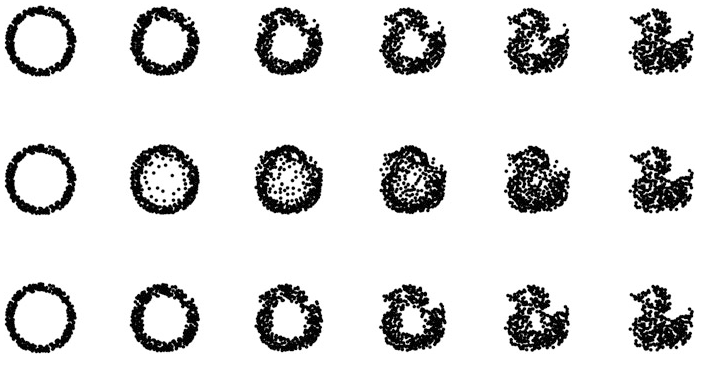
\includegraphics[width=\linewidth]{assets/ch05-fig-5-3.pdf}
\caption{环带上点分布与鸭形点分布之间的插值. 第一排按\autoref{fig:2.5}的方法计算指派，再让点以常速在起点与终点位置之间插值运动. 第三排使用实现距离$W_2$的最优指派作同样处理（因而得到$\mathbb W_2$中的测地线）. 第二排则通过极小化距离平方和，将插值计算为$\mathrm{SW}_2$的重心. 图片由J.~Rabin惠予提供，并改编自\cite{b256}.}\label{fig:5.3}\index{S140@切片Wasserstein距离（Sliced Wasserstein distance）|hyperpage}
\end{figure}

\begin{figure}[htbp]
\centering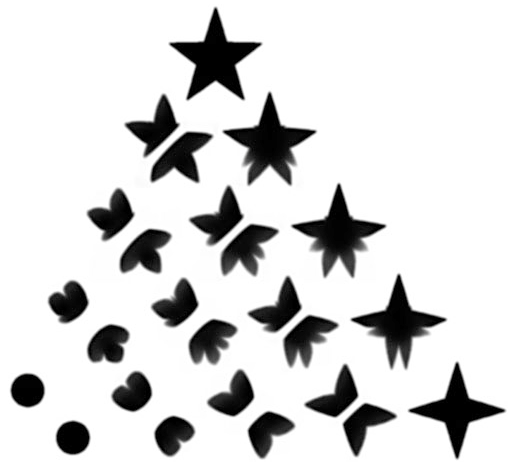
\includegraphics[width=.78\linewidth]{assets/ch05-fig-5-4.pdf}
\caption{三种不同形状（五角星、四角星及两个小圆盘的并）之间的插值. 每张图像表示在$\mathbb W_2$中计算的三个形状之间的一个重心. 图片由G.~Peyré惠予提供.}\label{fig:5.4}
\end{figure}
